\chapter{Results}\label{sec:results}
% In this chapter we expect you to list and explain all the results that you have achieved. Pictures can be useful to explain the results. Think about this chapter as something similar to the demo of the oral presentation. You can also include pictures about use-cases (you can also decide to add use cases to the high level overview chapter).

\section{Testing of the CamPUF}
[TODO: write]

\subsection{Dataset}\label{sec:dataset}
After some testing, this dataset was eventually chosen \cite{dataset_url}. It is composed of various sets of both RAW and JPEG images taken with five different 12-megapixel Sony IMX377 camera sensors, used by Google Nexus 5X smartphones \cite{dataset_explanation}. The key aspect in the preference of this dataset over the others tested is that all the RAW images are completely dark photos taken with the sensor lens fully covered. This is critical since the DSNU extraction efficiency is highly influenced by the presence of any light source exposed to the sensor.

Another advantage of choosing this dataset is that it was made with the purpose of testing another CamPUF implementation, having different relevant configuration ready to test, as for images taken in different room temperatures ($25^{\circ}$C, $35^{\circ}$C and $45^{\circ}$C). It is worth noting that for any real-world practical implementation, the images provided to the enrollment/authentication algorithm should be taken in a similar way, in RAW format and trying to cover the sensor lens as much as possible.

[TODO: referring to pictures below explain why newer sensor models could have less DSNU noise to rely on]

\begin{figure}[h!]
	\vspace{0.5cm}
	\includegraphics[width=\textwidth, height=5 cm]{example-image-a}
	\caption{This is the image \emph{caption}.}
	\label{fig:dataset}
\end{figure} 

\begin{figure}[h!]
	\vspace{0.5cm}
	\includegraphics[width=\textwidth, height=5 cm]{example-image-a}
	\caption{This is the image \emph{caption}.}
	\label{fig:dataset2}
\end{figure} 

\subsection{Setup}
The dataset was then thoroughly tested using a python script \emph{auto\_testing.py} that automated the following steps:

\begin{enumerate}
	\item Reading one or multiple images (and in this case, making the pixel-wide average).
	\item Obtaining the reference key after enrolling with that image.
	\item Trying to authenticate with a set of images, one after the other, by comparing the response key with the reference key generated from the previous step. If the Hamming Distance of the two keys is below a certain threshold, then the couple (\emph{enrollment image}, \emph{authentication image}) is said to be authenticated.
	\item After trying all the images combinations, the script computes the Hamming Distance average for the couple (\emph{enrollment image}, \emph{authentication set}).
\end{enumerate}

The main difference when picking the \emph{authentication set} to use is the source sensor of the images with respect to the source sensor of the \emph{enrollment image}. Two different cases are distinguished:

\begin{itemize}
	\item \textbf{Intra-Sensor} testing: both the \emph{enrollment image} and the \emph{authentication set} come from the same source sensor.
	\item \textbf{Inter-Sensor} testing: The \emph{enrollment image} and the \emph{authentication set} come from a different sensor.
\end{itemize}

\subsubsection{Parameters}
The main parameters used were generally:
\begin{itemize}
	\item \textbf{Key Length}: 256 bits, both for the reference key and the response key.
	\item \textbf{Hamming Distance Threshold}: 4 bits.
	\item \textbf{Number of Frames Averaged}: 5 frames for the enrollment, 1 frame for the authentication.
	\item \textbf{Number of Images tested for Authentication}: generally 50 for each run, 20 in the case of temperature testing. \ref{sec:temperature}
\end{itemize}

\subsubsection{Expected Results}

For the algorithm to be of any use, when testing \textbf{Intra-Sensor} couples it is expected to yield positive results on the authentication, meaning that the \emph{Intra-Sensor Hamming Distance} between the reference key and the response key must be low enough, ideally zero. This is needed in order to avoid any false negatives where devices are incorrectly unauthorized.

Another crucial assumption is related to the opposite case, where \textbf{Inter-Sensor} couples are expected to yield negative results on the authentication, meaning that the \emph{Inter-Sensor Hamming Distance} between the reference key and the response key must be high enough, in this case ideally around 50\% of the key length to match the expected Hamming Distance of two random bit sequences. Finally, this is also needed to avoid any false positives where devices are incorrectly authorized.

\subsection{Results}
The results were gathered after several runs of the \emph{auto\_testing.py} script. The results obtained from the testing process are in line with the expected outcomes, validating the effectiveness of the CamPUF implementation. The graph below presents the Hamming Distance percentages for different scenarios, considering 1 frame and 5 frames for both \textbf{Intra-Sensor} and \textbf{Inter-Sensor} testings:

\begin{figure}[h!]
	\centering
	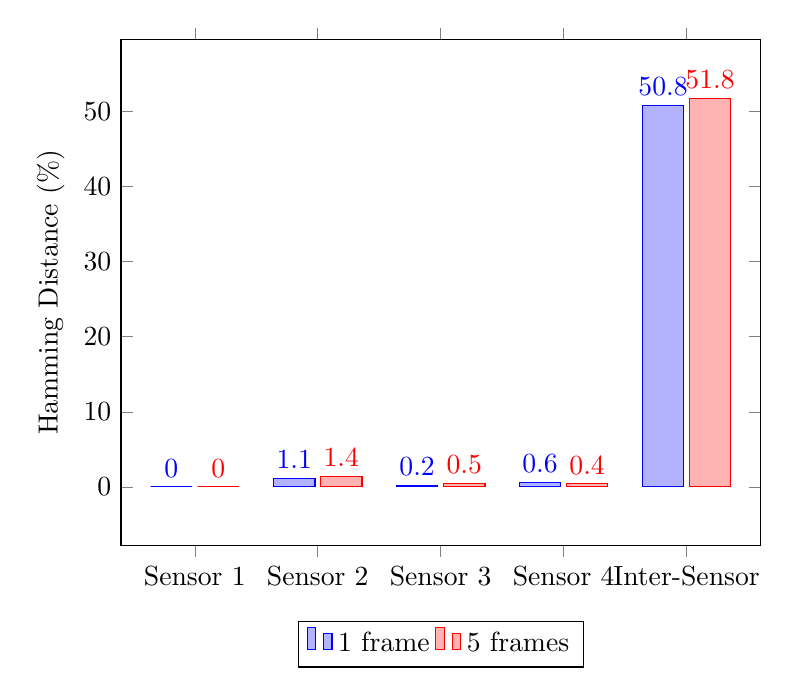
\begin{tikzpicture}
		\begin{axis}[
			width=0.8\textwidth,
			height=8cm,
			bar width=15pt,
			ybar,
			enlargelimits=0.15,
			legend style={at={(0.5,-0.15)},
			anchor=north,legend columns=-1},
			ylabel={Hamming Distance (\%)},
			symbolic x coords={Sensor 1, Sensor 2, Sensor 3, Sensor 4, Inter-Sensor},
			xtick=data,
			nodes near coords,
			nodes near coords align={vertical},
			]
			\addplot coordinates {(Sensor 1, 0.0) (Sensor 2, 1.1) (Sensor 3, 0.2) (Sensor 4, 0.6) (Inter-Sensor, 50.8)};
			\addplot coordinates {(Sensor 1, 0.0) (Sensor 2, 1.4) (Sensor 3, 0.5) (Sensor 4, 0.4) (Inter-Sensor, 51.8)};
			\legend{1 frame, 5 frames}
		\end{axis}
	\end{tikzpicture}
	\caption{Hamming Distance Percentages for Intra-Sensor and Inter-Sensor Testings}
	\label{fig:results_graph}
\end{figure}

As evident from the graph, the CamPUF algorithm performed exceptionally well in \textbf{Intra-Sensor} testing. Even with just one image for enrollment, the Hamming Distance between the reference key and the response key was found to be remarkably low. This demonstrates that a single image is sufficient to achieve accurate intra-sensor authentication, showcasing the efficiency of the algorithm.

Moreover, it was observed that a relatively low threshold of 4 bits is adequate to determine authentication success. This means that if the Hamming Distance falls below the threshold, the authentication process is successful. Fine-tuning this threshold allows for balancing between security and convenience. Lowering the threshold can increase security but may require more attempts to successfully authenticate. Conversely, increasing the threshold may reduce security but lead to faster and easier authentication.

The \textbf{Inter-Sensor} testing results align with expectations, showing Hamming Distances around 50\%, which is in line with the expected Hamming Distance between two random bit sequences. This confirms that CamPUF effectively discriminates between images taken from different sensors, providing a reliable mechanism to prevent unauthorized access.

In conclusion, the testing results demonstrate that the CamPUF implementation is capable of providing robust and accurate authentication.

\subsubsection{Temperature Resilience}

One critical aspect of the CamPUF implementation is its resilience to changes in temperature, which can impact the quality of sensor outputs. Higher temperatures often lead to increased random noise coming from the electrons inside the CMOS sensors, resulting in less noticeable DSNU noise that the algorithm relies on. We conducted testing under varying temperatures to assess the algorithm's performance in such scenarios.

The sensor tested for Intra-Sensor testing was Sensor 1, and the temperature changes refer to the room temperature relative to the images used for the authentication phase. The enrollment was always done with a room temperature of 25°C.

\begin{figure}[h!]
	\centering
	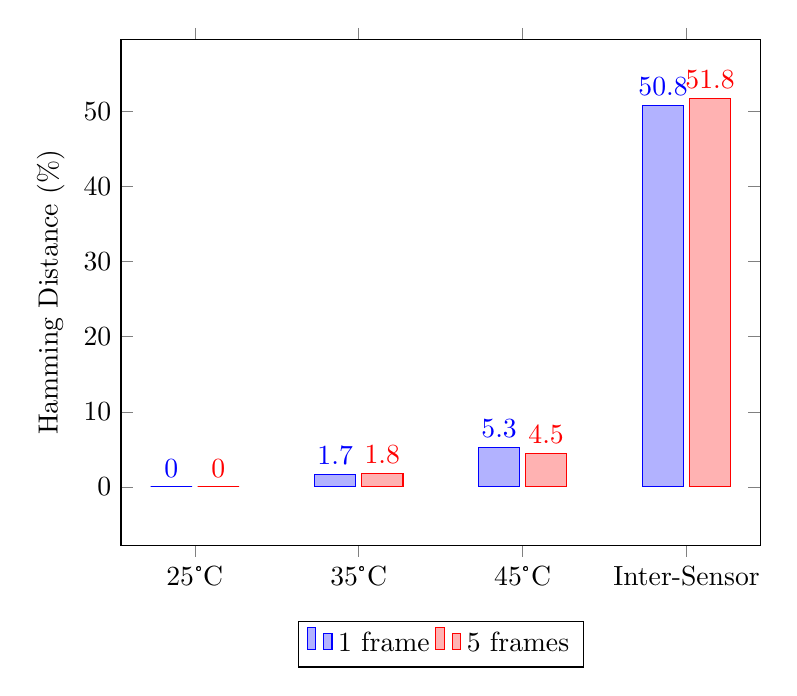
\begin{tikzpicture}
		\begin{axis}[
			width=0.8\textwidth,
			height=8cm,
			bar width=15pt,
			ybar,
			enlargelimits=0.15,
			legend style={at={(0.5,-0.15)},
			anchor=north,legend columns=-1},
			ylabel={Hamming Distance (\%)},
			symbolic x coords={25°C, 35°C, 45°C, Inter-Sensor},
			xtick=data,
			nodes near coords,
			nodes near coords align={vertical},
			]
			\addplot coordinates {(25°C, 0.0) (35°C, 1.7) (45°C, 5.3) (Inter-Sensor, 50.8)};
			\addplot coordinates {(25°C, 0.0) (35°C, 1.8) (45°C, 4.5) (Inter-Sensor, 51.8)};
			\legend{1 frame, 5 frames}
		\end{axis}
	\end{tikzpicture}
	\caption{Hamming Distance Percentages for Intra-Sensor and Inter-Sensor Testings at Different Temperatures}
	\label{fig:temperature_graph}
\end{figure}

As expected, the results show that the average Intra-Sensor Hamming Distance rises with increasing temperatures. At 25°C, the Hamming Distances remain negligible (0.0\%) for both one frame and five frames enrollments, indicating that even with minimal data, the algorithm achieves accurate authentication. However, at higher temperatures of 35°C and 45°C, the Intra-Sensor Hamming Distances slightly increase to 1.7\% and 5.3\% (for one frame enrollment), and 1.8\% and 4.5\% (for five frames enrollment), respectively.

Despite the slight increase in Intra-Sensor Hamming Distances with rising temperatures, they remain significantly low compared to the Inter-Sensor Hamming Distances, which are consistently around 50.8\% for one frame enrollment and 51.8\% for five frames enrollment. This highlights the algorithm's robustness and its ability to maintain reliable authentication even under varying temperatures.

In conclusion, the CamPUF implementation demonstrates promising temperature resilience. While the average Intra-Sensor Hamming Distance increases with higher temperatures, it remains negligible compared to the Inter-Sensor Hamming Distance. This reinforces the algorithm's effectiveness in providing secure and accurate device authentication across different environmental conditions.

\subsection{Attacks Mitigation}
TODO:

\section{Known Issues}
% If there is any known issue, limitation, error, problem, etc...explain it in this section. Use a specific subsection for each known issue. Issues can be related to many things, including design issues.
The main limitation of this implementation of CamPUF is the need for a dataset of images highly similar to the one used for testing described in \ref{sec:dataset}. Even if the TODO:


\section{Future Work}
% Adding a section about how to improve the project is not mandatory but it is useful to show that you actually understood the topics of the project and have ideas for improvements.
\label{sec:future_work}

